%&pdflatex
\chapter{Materials \& Methods}
Hanze template says I should link my GitHub repository somewhere at the start of this chapter, so here it is:
\href{https://github.com/denniswiersma/internship}{GitHub repository}

%&pdflatex
\begin{table}[H]
    \centering
    \begin{tabular}{|p{2.5cm}||p{2cm}|p{3cm}|p{5cm}|}
        \hline
        \textbf{Package} & \textbf{Version} & \textbf{Application} & \textbf{Reference} \\
        \hline
        \hline
        python & \verb| >3.12| & General purpose programming & \cite{python} \\
        \hline
        pandas & \verb|^2.1.3| & Data operations & \cite{python:pandas} \\
        \hline
        matplotlib & \verb|^3.8.1| & Plotting & \cite{python:plt} \\
        \hline
        seaborn & \verb|^0.13.0| & Plotting & \cite{python:sns} \\
        \hline
        rpy2 & \verb|^3.5.14| & Calling R code from within python & idk \\
        \hline
        scipy & \verb|^1.11.3| & used for some stuff in EDA, but is that even worth mentioning? & \cite{python:scipy} \\
        \hline
        scikit-learn & \verb|^1.3.2| & ML performance metrics & \cite{python:scikit-learn} \\
        \hline
        fastcluster & \verb|^1.2.6| & Faster hierarchical clustering & \cite{python:fastcluster} \\
        \hline
    \end{tabular}
    \caption{Python packages used in the project.}
    \label{tab:python_packages}
\end{table}


%&pdflatex
\begin{table}[H]
    \centering
    \begin{tabular}{|p{2.5cm}||p{2cm}|p{3cm}|p{5cm}|}
        \hline
        \textbf{Package} & \textbf{Version} & \textbf{Application} & \textbf{Reference} \\
        \hline
        \hline
        R & \verb|4.2.1| & Statistical programming & \cite{r} \\
        \hline
        Partykit & \verb|1.2-20| & Fitting trees \& forests & \cite{r:party1} \cite{ctree:art} \cite{r:party3} \\
        \hline
        glmnet & \verb|4.1-8| & Fitting a multinomial logistic model & \cite{r:glmnet1} \cite{r:glmnet2} \\
        \hline
        grDevices & \verb|4.2.1| & R's graphic devices for saving plots & \cite{r} \\
        \hline
    \end{tabular}
    \caption{R packages used in the project.}
    \label{tab:r_packages}
\end{table}


\section{Materials}

[Describe the data you used, how you got it, and its structure.]
[Describe how the original data was changed for your project.]
[Describe used software tools and libraries with name, version, usage goal, and reference. Can be done in a table.]

[Define response (cancer type annotations) and covariates (TCs) early and clearly]
[Since it will be a part of methods, keep things short and clear]

\subsection{Data acquisition}
The data for this project was provided by the Fehrmann group at University Medical Center Groningen.
Data acquisition was performed by this group as described by \cite{bhat:cna} and will be summarised here:

Data was collected from The Cancer Genome Atlas (TCGA), consisting of 10817 samples generated with RNA sequencing. [is this number results?]
This data underwent quality control and pre-processing.

PCA whitening was applied on the pre-processed TCGA dataset, resulting in uncorrelated covariates that each have a variance of one.
The whitened data's covariance matrix is then equal to the identity matrix, which speeds up the convergence rate in the application of the consensus-ICA (c-ICA) algorithm.

% \subsubsection{Independent Component Analysis}
% [Explain what ICA is, how does it work, and especially what does it do in this context.]
[Expand on ICA]
C-ICA was then applied to the dataset, separating the gene expression profiles into Independent Components (ICs).

This method results in a set of ICs, in this context called Transcriptional Components (TCs), which represent activity scores of genes in each TC, as well as a mixing matrix.
The latter represents the degree to which TCs are present in a given sample.

Corrections were applied to the mixing matrix using a Johnson transformation to mitigate platform specific and batch effects, therefore only leaving biological influences.





\subsection{Data preprocessing}

The TCGA mixing matrix, henceforth just called mixing matrix, and its annotation data are each loaded into a \verb|pandas| data frame.
An inner join is applied to these data frames using sample names as their common denominator.
This join operation removes samples that do not have an annotation from the mixing matrix, resulting in a single data frame containing the covariates and a column with the response variable.
Prior to the join operation, the mixing matrix consisted of 10817 samples and after 8862 were left. [numbers are results]

In general, the dataset is randomly split into a training, testing, and validation set using stratified sampling.
This is done by first splitting the data into a training set and a temporary set, then splitting the latter of these into testing and validation sets.
An exception to this is process is discussed in \fref{sec:methods:glmnet}.







\section{Methods}
Describe existing methods and their relevance.
Goal of using the software, its application, what parameters.
Figures and flowcharts might help.
Describe statistical methods to determine significance of outcomes.

[Small introduction on why first glmnet, then trees, then forests here?
Then have the actual description in the subsections below?]







\subsection{Generalised Linear Models using Elastic Net Regularisation} \label{sec:methods:glmnet}
% Why is it important to make it so there are "no more" correlated predictors in the data though?
% Applying regularisation methods is beneficial as it functions as a means of feature selection where the influence of TCs with very similar effects are combined, and TCs that do not influence the prediction are not used.
% In traditional regression models, correlated predictors can cause high variance of the weight vector.
% For the model to be stable, we need the variance of the weight vector to be low because much more mathematics.
% When the predictors are highly correlated, the variance can be / is high and therefore our model can be unstable. [https://towardsdatascience.com/why-exclude-highly-correlated-features-when-building-regression-model-34d77a90ea8e] Should probably find a better source for that.
Logistic regression techniques offer an interpretable way of classifying data.
[Need something to glue these together]
While TCs are statistically independent, the activity scores in the mixing matrix are not, introducing the problem of multicollinearity.
Regularisation techniques, like lasso, ridge, and elastic net regression, may be applied in order to handle this problem. \cite{glmnet:reg}

The \verb|glmnet| package implements such regularisation techniques and was therefore used to fit a Generalised Linear Model with its option for multinomial models.
This specific implementation offers elastic net regularisation controlled by a single parameter value between zero (ridge) and one (lasso).
The former of these two techniques shrinks the influence of TCs with very similar effects, while the latter would pick one TC and discard the others in the same scenario. [cite glmnet]
Setting the parameter to a value in between results in the combination of these techniques, referred to as elastic net regularisation.

The minimum mean cross-validated error, \verb|lambda.min|, was calculated using tenfold cross validation by running the \verb|cv.glmnet| function.
The value found for \verb|lambda.min| was used to fit a model using the \verb|glmnet| function.
The parameters which deviated from their defaults are shown in \fref[plain]{tab:glmnet_conv_reg} for both functions.

%&pdflatex
\begin{figure}[htp]
    \centering
    \textbf{This is a beautiful figure title}\par\medskip
    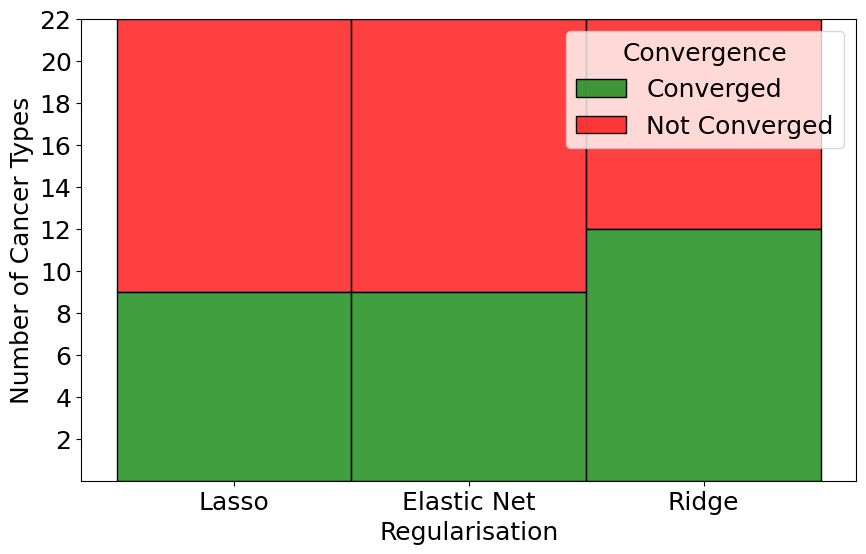
\includegraphics[scale=0.45]{glmnet_conv_reg_18pt}
\caption{blablabla}
\label{fig:glmnet_conv_reg}
\end{figure}


In a process of iterative parameter adjustment the values for the \verb|alpha|, \verb|maxit|, and \verb|thresh| parameters were adjusted.
To ensure model convergence, cancer types with fewer than one hundred samples were removed from the dataset.
A subset of 250 randomly chosen samples from two randomly chosen cancer types was made and split into training, testing, and validation sets at a ratio of 70\%, 15\%, and 15\% respectively.
The \verb|glmnet| package was used as described above to fit a model.
Additional cancer types were added to the [sample space? That is a cool big boy word, but I don't know if it is correct in this context] until the model stopped converging, resulting in a maximum number of cancer types with which the model would work.

To increase this maximum number of usable cancer types a similar process was [performed].
The static total of 250 randomly chosen samples was replaced by randomly choosing 100 samples for every cancer type in the training set.
Samples not present in the training set were placed in the testing set, only for cancer types currently in the dataset.
The process was started by selecting two random cancer types and 100 of their samples.
Cancer types, and therefore samples, were iteratively added to the dataset until the model stopped converging, at which point the number of samples per cancer types was reduced until the convergence was achieved once again, utlimately reaching an optimum number of cancer types and samples per cancer type.
This optimum data shape was used for the final \verb|glmnet| model.

To summarise, the following method was used until an optimum was found:
\begin{enumerate}
    \item Remove cancer types with fewer than 100 samples from the dataset.
    \item Randomly select two cancer types and 100 samples for each cancer type and place them in the training set.
    \item Place the remaining samples for these cancer types in the testing set.
    \item Run \verb|cv.glmnet| with the parameters found in \fref[plain]{tab:glmnet_conv_reg}.
    \item Run \verb|glmnet| with parameters found in \fref[plain]{tab:glmnet_conv_reg}.
    \item[6a.] If the model converges:
        \begin{itemize}
            \item Add a cancer type, and therefore an additional 100 samples, to the dataset.
            \item Return to step 3.
        \end{itemize}
    \item[6b.] If the model does not converge:
        \begin{itemize}
            \item Reduce the number of samples per cancer type by one.
            \item Return to step 3.
        \end{itemize}
\end{enumerate}

The optimal values found during this process can be found in \fref{sec:results:glmnet}





\subsection{Conditional Inference Trees}
Decision trees were chosen as they tend to require little data preparation, while still being relatively easy to interpret as compared to methods like deep learning \cite{ctree:trees_good}.
Most well known decision trees, like CART and C4.5, utilise an information measure such as Gini index or information gain.
However, these implementations tend to overfit \cite{ctree:overfit}, requiring pruning, and introduce a bias towards TCs with many possible splits \cite{ctree:bias}.

Conditional inference trees were chosen in particular for their approach to overfitting and selection bias problems, as described by \cite{ctree:art}.
The algorithm starts by testing the global null hypothesis made up of partial hypotheses stating that the conditional distribution of the cancer types given a particular TC, is equal to the conditional distribution of the cancer types.
This is formulated by \cite{ctree:art} as $H_0^j : D(\mathbf{Y}\vert X_j) = D(\mathbf{Y})$.
Thus, when this partial null hypothesis is accepted one may infer that none of the remaining covariates are significantly associated with the response.

If all partial null hypotheses are rejected, the global null hypothesis may be rejected as well.
In this case, the algorithm proceeds by measuring the association between the cancer types and each TC.
The dataset is split on the TC with the strongest association to the cancer types.

The dataset was split into a training (70\%), testing (15\%), and validation (15\%) sets, after which the \verb|partykit| package's \verb|ctree| function was used to fit conditional inference trees.

To assess performance using multiple data points, a limited grid search was performed.
A tree was fit for each set of parameters found in \fref{tab:ctree_params}.
These parameters were chosen after a short literary review where \cite{gs:a}, \cite{gs:alpha2}, and \cite{gs:a_maxdepth} mention changing the value for \verb|alpha|.
\cite{gs:minsplit} changes the \verb|minsplit| parameter and \cite{gs:minbucket} changes the \verb|minbucket| parameter.
\cite{gs:def_bon}, \cite{gs:def_a_bon}, and \cite{gs:def_a_minsplit_minbucket} say they use default values for the parameters they mention.

Desiring a stable significance level, \verb|alpha| was kept at its default value of 0.05, while \verb|minsplit| and \verb|minbucket| were selected as parameters to vary.
Values for these parameters were chosen by doubling and halving the default values, resulting in the aforementioned \fref{tab:ctree_params}.

%&pdflatex
\begin{table}[H]
    \centering
    \begin{tabular}{|p{3cm}|p{3cm}|}
        \hline
        \texttt{minsplit} & \texttt{minbucket} \\
        \hline
        \hline
        10 & 7 \\
        20* & 7* \\
        30 & 7 \\
        20 & 3 \\
        20 & 14 \\
        \hline
    \end{tabular}
    \caption{Values used for paramaters in conditional inference tree gridsearch. Default values are indicated with *.}
    \label{tab:ctree_params}
\end{table}


[Some closing remark]

\subsection{Conditional Inference Forests}
Ensemble methods tend to improve performance of [something something]

The \verb|partykit| package offers an implementation of a random forest, using conditional inference trees as base learners, in the form of the \verb|cforest| function.
This function differs from more common random forest implementations by its aggregation method, described by \cite{cforest:agg}, and its randomisation method.
In order to produce differing trees, the algorithm randomly selects a subset of TCs for splitting in every node of every tree, where the more common implementations only do this for every individual tree.

The forest's performance was assessed similarly to the conditional inference trees.
An additional parameter, \verb|ntree|, specifying the number of trees in the forest was added to the limited grid search.

%&pdflatex
\begin{table}[H]
    \centering
    \begin{tabular}{|p{3cm}|p{3cm}|p{3cm}|}
        \hline
        \texttt{ntrees} & \texttt{minsplit} & \texttt{minbucket} \\
        \hline
        \hline
        10 & 10 & 7 \\
        10 & 20* & 7* \\
        10 & 30 & 7 \\
        10 & 20 & 3 \\
        10 & 20 & 14 \\
        50 & 20 & 7 \\
        \hline
    \end{tabular}
    \caption{Values used for paramaters in conditional inference forest grid search. Default values are indicated with *.}
    \label{tab:cforest_params}
\end{table}


[How do I say I did a more extensive grid search because the forest performed better than the trees, without touching on results in this methods section?]
More possible values for all parameters were included, while also incorporating the \verb|testtype| parameter.
The many trees in the forest should make a multiple testing correction redundant, and could possibly even harm performance.
[We wanted to confirm this]
The parameters used for this grid search can be found in \fref{tab:cforest_params_large}.

%&pdflatex
\begin{table}[H]
    \centering
    \begin{tabular}{|p{3cm}|p{3cm}|}
        \hline
        \textbf{Parameter} & \textbf{Values} \\
        \hline
        \hline
        \multirow{2}{*}{\texttt{testtype}} & bonferroni \\
        & univariate \\
        \hline

        \multirow{5}{*}{\texttt{ntrees}} & 5 \\
        & 10 \\
        & 100 \\
        & 500 \\
        & 1000 \\
        \hline

        \multirow{4}{*}{\texttt{minbucket}} & 3 \\
        & 7 \\
        & 14 \\
        & 35 \\
        \hline

        \multirow{3}{*}{\texttt{minsplit}} & 10 \\
        & 20 \\
        & 50 \\
        \hline
    \end{tabular}
    \caption{Values used for paramaters in conditional inference forest grid search.}
    \label{tab:cforest_params_large}
\end{table}


% Testtype was also changed because the default for the tree is Bonferroni (multiple testing correction) while the default for the forest is univariate.
% Apparently the many trees in the forest pretty much eliminate the need for multiple testing correction(?) and there should be some rational in the cforest paper.

% It makes differing trees my randomly choosing a subset of variables which it will consider for splitting. This is the mtry parameter. The default value is the square root of the number of variables.
% https://academic.oup.com/biostatistics/article/7/3/355/248945?login=false





\subsection{Performance Metrics}
[How would this be a section in results? Maybe incorporate in some other parts?]
A collection of performance metrics was selected to assess the performance of each fitted model.
The implementation in the \verb|scikit-learn| Python package's \verb|metrics| module were used for all four measures.

\subsubsection{Top-k Accuracy}
Accuracy is a simple measure of the fraction of correctly classified instances.
While easy to interpret, accuracy does not consider whether an instance is [something something] \cite{acc:bad}
Alternatively, top-k accuracy is used, including the k most probable predictions in its measure.
While still suffering from some of the same issues as accuracy, it provides some insight into whether a model was close to the correct answer. [cite paper?]

[The implementation of this metric in the \verb|sklearn.metrics.top_k_accuracy_score| function was used for calculations].

\subsubsection{Area Under the Curve}
Area Under the Curve of the Receiver Operating Characteristic curve (AUC ROC) summarises the True Positive (TP) rate and False Positive (FP) rate into a single number.
Although AUC ROC does not consider True Negative or False Negative classifications, it still provides valuable insight into a model's behavior.
[Expand and cite paper]

The \verb|sklearn.metrics.roc_auc_score| function was used to calculate AUC ROC with the \verb|multi_class| parameter set to \verb|ovr|, or one-versus-rest.

\subsubsection{Matthews Correlation Metric}
The Matthews Correlation Metric (MCC) provides insight into the True Negative (TN) rate and False Negative (FN) rate \cite{mcc:paper} which AUC ROC lacks.
The MCC was made considering a scenario with just two classes.
To apply this metric to the multi-class problem at hand, one might force it into such a shape by labeling instances as part of or not part of a group.
Instead, an extension of the MCC described by \cite{mcc:multi} was used.

The implementation of MCC in the \verb|sklearn.metrics.matthews_corrcoef| function was used.

[Can't think of much else to say right now. Come back to this later]

% The MCC metric can be described as a more well-rounded version of the F1 score, since it includes the influence of TN classified instances, which the latter metric does not. [cite paper]
% \href{https://www.sciencedirect.com/science/article/abs/pii/S1476927104000799}{paper on extending MCC to multiclass problems}
% \href{https://towardsdatascience.com/matthews-correlation-coefficient-when-to-use-it-and-when-to-avoid-it-310b3c923f7e}{Medium article on MCC}
% "MCC is high only if your classifier is doing well on both the negative and positive elements"


\subsubsection{Adjusted Rand Index}
The Adjusted Rand Index (ARI) is a measure for the similarity of two clusters by considering all pairs of samples. \cite{ari:rand}
The raw Rand Index is adjusted for chance by [read and cite paper] \cite{ari:adj}
\href{https://sci-hub.ru/10.1007/bf01908075}{comparing partitions paper}

[cool, what is the benefit?]


\subsection{Model selection}
[maybe just mention how your choose the model (mcc) and why that way in the next chapter. Entire chapter unneeded]


We then took the model that has the highest overall MCC. [<- Is that the same one as all the highest points in the violin plots?]
[Okay, apart from this sentence, what else is there to say that isn't results? Maybe combine performance metrics and this into a single section?]


\subsection{Validation on microarray data}
In order to [do what exactly? Explain (probably in more than half a sentence)] the model is validated by having it predict on samples from a microarray platform.

[The idea of removing platform specific and batch effects should probably be introduced in ... well, the introduction. Feels a bit out of place to suddenly switch to this aspect here.]

Like with the TCGA dataset, a mixing matrix based on microarray data was acquired from the Fehrmann group.
Their data acquisition is likewise described by \cite{bhat:cna}.
Microarray expression data was acquired from GEO platform GPL570 containing 21592 samples.
A similar quality control and pre-processing [...] was applied.
The TCs from the TCGA dataset are then projected onto the GPL570 dataset, resulting in a mixing matrix representing the degree to which the TCGA TCs are present in the GPL570 dataset.
This GPL570 mixing matrix is then corrected using a Johnson transformation.



\subsection{Variable Importance}
[something something filter data and train new forests]

Variable importance scores for these models were calculated using the \verb|partykit| package's \verb|varimp| function with default settings.
This function determines importance scores by calculating the mean decrease in out of bag accuracy.
[This is done] by calculating an accuracy score before and after permuting a given [covariate/TC] and comparing the results.
